\documentclass[11pt, a4paper]{article}
\usepackage[utf8]{inputenc}
\usepackage{amsmath, amssymb}
\usepackage{graphicx}
\usepackage{booktabs}
\usepackage{geometry}
\usepackage{tikz}
\usetikzlibrary{positioning, arrows.meta}
\geometry{margin=1in}
\usepackage{hyperref}

\title{\textbf{Synthetic Intelligence Requires Exact Memory:\\ A Dual-Layer Architecture for Trustworthy Agency}}
\author{Sciencedelic Metatech Research}
\date{\today}

\begin{document}
\maketitle

\begin{abstract}
Current Artificial Intelligence (AI) architectures conflate fuzzy reasoning with fuzzy memory, leading to "silent-wrong" answers and the "Fried Brain Effect". We propose the term \textbf{Synthetic Intelligence (SI)} to distinguish synthetic execution from biological heuristics. SI requires exact math for memory and fuzzy math for reasoning. We demonstrate that the exact memory layer is independently validated: the Recallspection architecture achieved Level L4 on the Agent Memory Integrity (AGMI) benchmark. To prove this architecture functions end-to-end, we present \textbf{FlightSpection}, a reference integration that bridges exact memory with an order-invariant reasoning engine. In 1,000 trials, a naive vector store produced 11.4\% silent-wrong answers. FlightSpection produced 0\% silent-wrong answers at a 52\% refusal rate.
\end{abstract}

\section{Introduction}
\subsection{The Naming Problem}
The term "Artificial Intelligence" (AI), coined in 1956, uses "artificial" to mean fake. This is a semantic error. A synthetic diamond is a real diamond. We introduce \textbf{Synthetic Intelligence (SI)} to denote non-biological systems that use exact math for memory.

\subsection{The Human Cost: The Fried Brain Effect}
Because current AI cannot be trusted with exact data, humans must act as the out-of-band memory layer. Managing multiple agents requires constant context switching, causing cognitive overload. We define this as the \textit{Fried Brain Effect}.

\subsection{The Contract: Exact First}
We propose a strict architectural contract for SI: \textit{Exact first, fuzzy proposes, caller verifies.} The system must return either the exact value or an explicit tamper error ($Err(Tamper)$), never a silent wrong answer.

\section{Technical Architecture and Validation}
\begin{figure}[h]
\centering
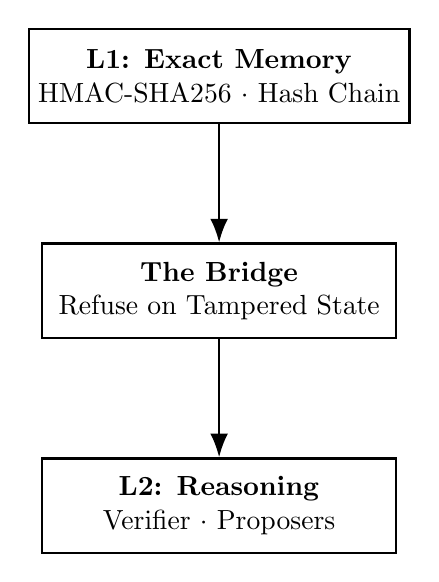
\begin{tikzpicture}[
  node distance=1.5cm,
  box/.style={rectangle, draw=black, thick, align=center, minimum width=4.5cm, minimum height=1.2cm},
  arrow/.style={-{Latex[length=3mm]}, thick}
]
\node[box] (l1) {\textbf{L1: Exact Memory}\\HMAC-SHA256 \(\cdot\) Hash Chain};
\node[box, below=of l1] (bridge) {\textbf{The Bridge}\\Refuse on Tampered State};
\node[box, below=of bridge] (l2) {\textbf{L2: Reasoning}\\Verifier \(\cdot\) Proposers};
\draw[arrow] (l1) -- (bridge);
\draw[arrow] (bridge) -- (l2);
\end{tikzpicture}
\caption{The Dual-Layer SI Architecture.}
\end{figure}

\subsection{L1: Recallspection and AGMI Validation}
The L1 memory layer uses HMAC-SHA256 tags and a SHA-256 hash chain. This architecture achieved a \textbf{Level L4 rating} on the AGMI suite, rejecting 9/9 adversarial attacks (including rollback and truncation).

\subsection{L2: Orderspector Reasoning Layer}
The L2 layer contains a formal verifier and static proposers. The verifier acts as a hard ceiling. The proposer tier is fail-closed.

\subsection{The Bridge: FlightSpection}
FlightSpection enforces a strict rule: reasoning refuses to run on tampered rules. If the L1 store detects a cryptographic mismatch, the L2 engine halts.

\subsection{End-to-End Results}
\begin{table}[h]
\centering
\caption{End-to-end silent-wrong elimination (E13).}
\begin{tabular}{@{}lrr@{}}
\toprule
\textbf{Metric} & \textbf{Naive Store} & \textbf{FlightSpection} \\
\midrule
Total Trials & 1,000 & 1,000 \\
\textbf{Silent-Wrong Rate} & \textbf{11.4\%} & \textbf{0.0\%} \\
Refusal Rate (Safety Gate) & 0\% & 52\% \\
\bottomrule
\end{tabular}
\end{table}

\section{Limitations and Future Work}
FlightSpection handles 3 of the 6 anchors required by Raell's Stack Theorem. The remaining 3 (Authority, Causal, Norm) require external oracle mechanisms (Exospection).

\begin{thebibliography}{9}
\bibitem{synthetic_intelligence}
Sciencedelic Metatech. (2026). \textit{Synthetic Intelligence Requires Exact Memory}. Zenodo. 
\url{https://doi.org/10.5281/zenodo.23378369}

\bibitem{agmi}
Agent Memory Integrity (AGMI). (2026). \textit{L4 Conformance Result}. 
\url{https://agentmemoryintegrity.org/}
\end{thebibliography}
\end{document}